\chapter{High-Level and Low-Level Design}\label{chap:6}
\label{chap:design}
\noindent This chapter describes how the methodology of Chapter~\ref{chap:approach} is realised as software. It moves from the high level to the low level: first an overview of the system and the considerations that shaped its design, then the architecture of the whole system and of each subsystem, the strategies behind the main architectural decisions, the class diagram, and finally the policies and tactics that govern implementation, testing and maintenance.

\section{System Overview}\label{sec:6.1}
\label{sec:sysoverview}
\noindent The NIDPS is a self-contained security appliance built from software on a single Linux host. The host replaces the role of the home router's wireless network: clients connect to the NIDPS access point, and the NIDPS routes their traffic, through its own NAT, to the existing ISP router, which keeps handling the internet connection. No change is needed on client devices or on the ISP router.

\noindent Functionally, the system does five things:
\begin{enumerate}
    \item \textbf{Provides network access:} a wireless access point with DHCP, DNS and routing.
    \item \textbf{Inspects traffic:} inline signature inspection of every packet, plus flow-level analysis of all traffic, including encrypted traffic through metadata.
    \item \textbf{Decides:} fuses signature, anomaly and classification results into a per-flow verdict and a per-host risk score.
    \item \textbf{Responds:} blocks offending addresses automatically for a limited, escalating time.
    \item \textbf{Reports and stays available:} shows live statistics and alerts on a web dashboard, and keeps the network in a defined state when a component fails.
\end{enumerate}

\noindent The system is made up of independent services connected by a local event bus, rather than as one large program. The packet-forwarding path is kept as short as possible (kernel plus Suricata), and everything slower like machine learning, the database and the dashboard, sits beside that path instead of in it. Sections~\ref{sec:sysarch} and~\ref{sec:archstrategies} explain this choice in detail.

\section{Design Considerations}\label{sec:6.2}
\label{sec:designconsiderations}
\noindent This section records the assumptions, constraints, goals and development methods that shaped the design.

\subsection{Assumptions and Dependencies}\label{sec:6.2.1}
\label{sec:assumptions}
\begin{itemize}
    \item \textbf{Hardware:} the host is a mid-range laptop or a Raspberry Pi with at least 4\,GB of RAM, a wireless adapter that supports AP mode and an Ethernet port for the uplink.
    \item \textbf{Operating system:} Debian based Linux distribution with systemd, iptables (use of nftables is accepted, but not required), ipset (use of NFQUEUE is accepted, but not required) and support in the kernel.
    \item \textbf{Network position:} NIDPS is the only wireless network clients access. Devices which are connected directly to the ISP router via cable or directly by the ISP router's Wi-Fi are not protected. Turning off the ISP router's WiFi is a part of the set-up process.
    \item \textbf{Third-party software:} Suricata 7 or later with Emerging Threats Open ruleset, hostapd, dnsmasq, Python 3.11+ with scikit-learn and XGBoost. Periodic Internet access is required for ruleset updates.
    \item \textbf{End users:} Owner is NOT a security expert. Defaults should be safe and not require tuning, and dashboard should provide information about alerts in easy-to-understand terms.
    \item \textbf{Trust:} The NIDPS host and the admin's devices are trusted. The ISP router is assumed to be working, but is not trusted to provide any security.
    \item \textbf{Likely changes:} Changes are likely to include new attack types and new rules, models may be retrained and the TLS fingerprinting method could change from JA3 to its successor JA4, as TLS client libraries start to shuffle the order of extensions. Each of these is isolated by the design behind its component.
\end{itemize}

\subsection{General Constraints}\label{sec:6.2.2}
\label{sec:constraints}
\noindent Table~\ref{tab:constraints} lists the global constraints and their impact on the design.

\begin{table}[H]
\centering
\caption{General constraints and their impact on the design.}
\label{tab:constraints}
\begin{tabular}{|>{\raggedright\arraybackslash}p{0.18\linewidth}|>{\raggedright\arraybackslash}p{0.2\linewidth}|>{\raggedright\arraybackslash}p{0.5\linewidth}|}
\hline
\textbf{Constraint} & \textbf{Source} & \textbf{Impact on the design} \\
\hline
Limited CPU and memory & Low-cost target hardware & Tree-based models instead of deep networks; per-flow rather than per-packet ML; incremental feature statistics; rule groups trimmed to the home-network scope \\
\hline
Inline position & The NIDPS forwards all traffic & Forwarding path kept to kernel + Suricata; ML runs off-path; failure mode enforced in the kernel \\
\hline
Encrypted traffic & Most traffic uses TLS/QUIC & No payload inspection for ML; detection from flow metadata and JA3/JA3S only \\
\hline
Privacy & Household traffic is personal & No decryption; no payload storage; only flow metadata and alerts are kept, with a retention limit \\
\hline
Availability & A home network must not go down & Configurable fail-open default; block rate limits; allowlist; ipset entries that expire \\
\hline
Interoperability & Training data and live traffic must match & One flow extractor used offline and online; model files carry their feature schema \\
\hline
Security of the device & The NIDPS is itself a target & Dashboard bound to the LAN only, authenticated, management traffic allowlisted; services run without root where possible \\
\hline
Testability & Attacks cannot be run on real users & Isolated lab network and attacker machine for all attack tests \\
\hline
\end{tabular}
\end{table}

\subsection{Goals and Guidelines}\label{sec:6.2.3}
\label{sec:goals}
\begin{enumerate}
    \item \textbf{Never make the network worse than a plain router.} Every design choice is checked against this. It is why fail-open is the default, why blocks expire and why the number of blocks per minute is capped.
    \item \textbf{Keep the fast path short (KISS).} Only the kernel and Suricata sit in the forwarding path. Anything that can be done after the fact is moved off it.
    \item \textbf{Defence in depth.} No single detector is trusted to catch everything; each layer covers a weakness of the others (Section~\ref{sec:overview}).
    \item \textbf{Speed over memory where the two conflict, within a fixed budget.} Models and rule sets are loaded fully in memory to avoid disk access during inspection, but their size is capped to fit the hardware.
    \item \textbf{Explainable decisions.} Every block records which layer decided, why, and with what evidence, so the owner can trust or override it.
    \item \textbf{Same code for training and serving.} Features are computed by one implementation to rule out train/serve skew.
    \item \textbf{Configurable, safe defaults.} Thresholds, failure mode and block durations are configurable, but the defaults work without tuning.
\end{enumerate}

\subsection{Development Methods}\label{sec:6.2.4}
\label{sec:devmethods}
\noindent The project follows an iterative, incremental approach in short sprints of two weeks, aligned with the FYP milestones. Each increment delivers a working vertical slice: first the access point with Suricata (Layer 1, completed), then flow extraction and Layer 2, then Layer 3, then fusion and enforcement, and finally the watchdog and dashboard. This order means the system protects the network from the first increment onwards and every later layer can be measured against a working baseline.

\noindent The machine learning work follows the CRISP-DM cycle (data understanding, preparation, modelling, evaluation, deployment), because model quality depends on several rounds of data cleaning and re-evaluation. A plain waterfall model was considered and rejected: detection performance on real traffic cannot be known in advance, so requirements such as thresholds and feature sets must be allowed to change as results come in.

\section{System Architecture}\label{sec:6.3}
\label{sec:sysarch}
\noindent The system is decomposed into five runtime subsystems on the NIDPS host and one offline subsystem used for training. Figure~\ref{fig:architecture} shows the external architecture (how the NIDPS sits between clients, the ISP router and the administrator) together with the internal subsystems and their main data flows.

\begin{figure}[!htbp]
    \centering
    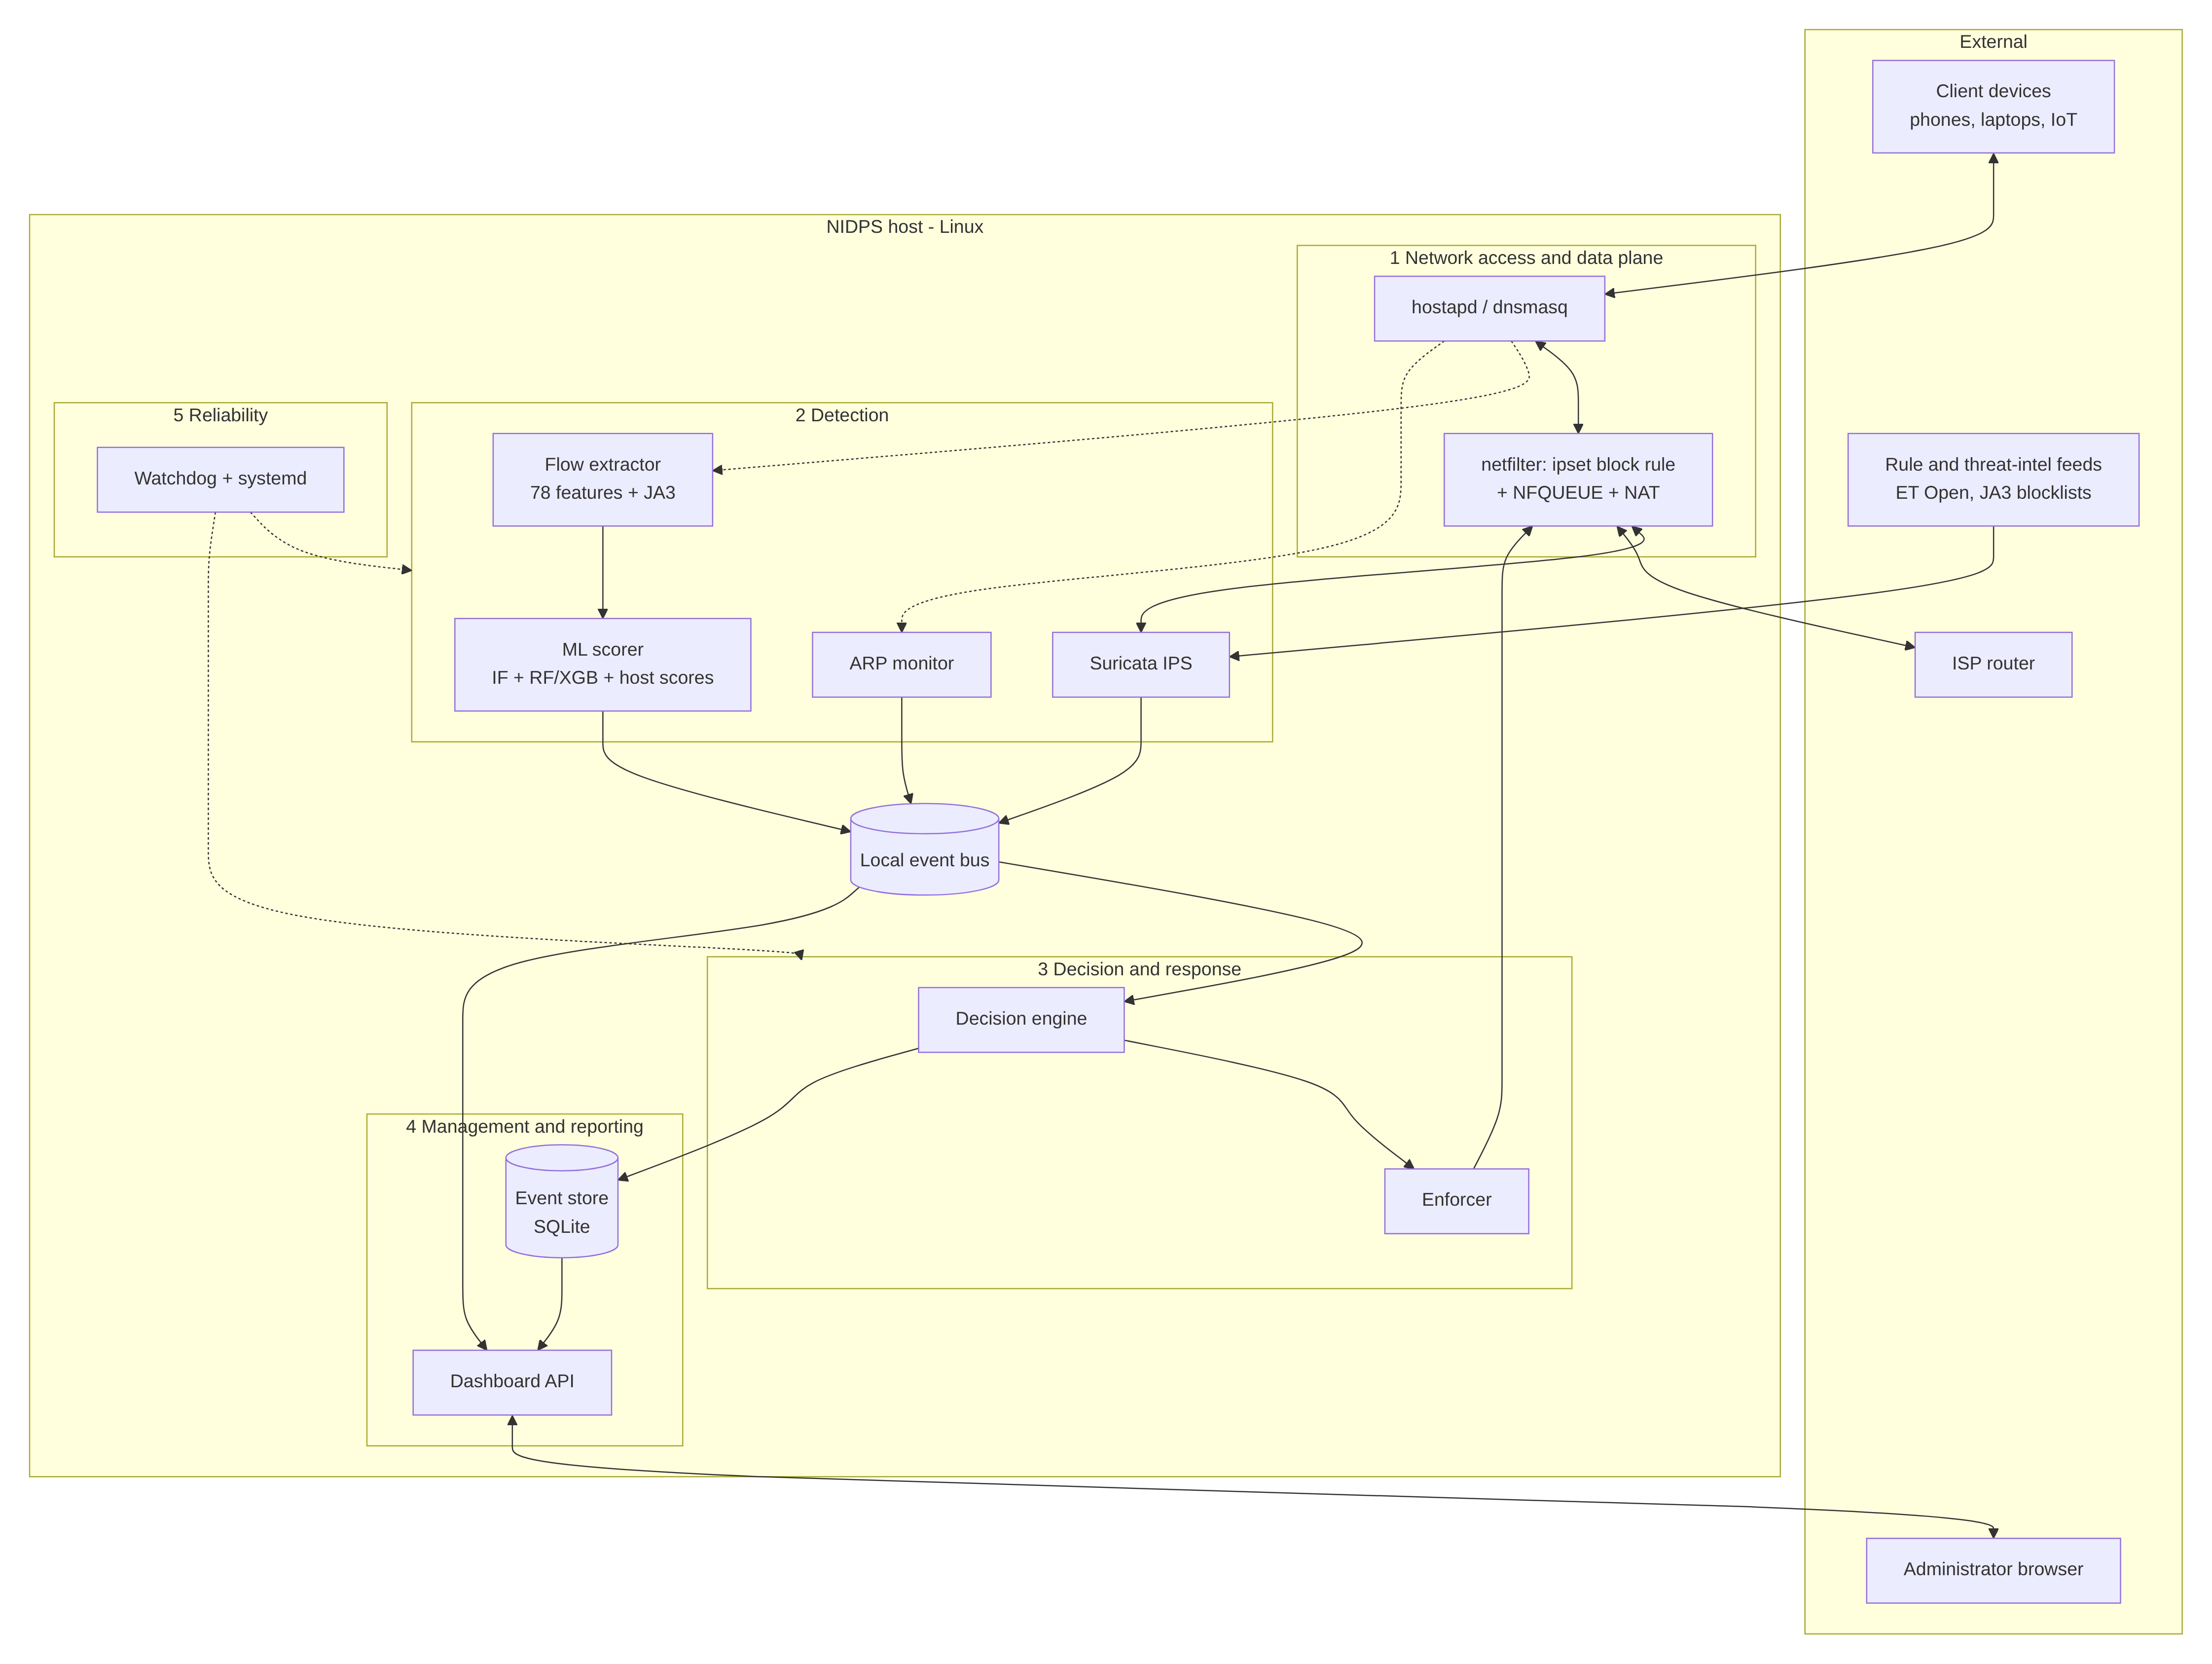
\includegraphics[width=\textwidth]{Figures/nidps_fig6_1.png}
    \caption{System architecture of the NIDPS.}
    \label{fig:architecture}
\end{figure}

\noindent The responsibilities are partitioned as shown in Table~\ref{tab:subsystems}.

\begin{table}[H]
\centering
\caption{Subsystem responsibilities.}
\label{tab:subsystems}
\begin{tabular}{|>{\raggedright\arraybackslash}p{0.22\linewidth}|>{\raggedright\arraybackslash}p{0.38\linewidth}|>{\raggedright\arraybackslash}p{0.28\linewidth}|}
\hline
\textbf{Subsystem} & \textbf{Responsibility} & \textbf{Main components} \\
\hline
1. Network access and data plane & Provide Wi-Fi, addressing and routing; hold the inline queue; enforce blocks and failure mode in the kernel & hostapd, dnsmasq, netfilter (iptables, ipset, NFQUEUE, NAT) \\
\hline
2. Detection & Produce evidence: signature alerts, ARP alerts, flow records, anomaly scores, class probabilities & Suricata, ARP monitor, flow extractor, ML scorer \\
\hline
3. Decision and response & Turn evidence into verdicts and host risk; apply and expire blocks & Decision engine, enforcer \\
\hline
4. Management and reporting & Store events; expose live statistics, alerts and configuration to the admin & Event store, dashboard API and web UI, configuration manager \\
\hline
5. Reliability & Detect failed or overloaded components; restart them; apply failure mode; record recovery metrics & Watchdog, systemd units \\
\hline
Offline: training & Regenerate datasets, train and validate models, publish versioned model files & Dataset builder, trainer, model registry \\
\hline
\end{tabular}
\end{table}

\noindent The subsystems collaborate through two channels. The forwarding path is purely in the kernel and Suricata, with a single feedback loop from the enforcer into ipset. All other communication goes through the local event bus: detectors publish evidence, the decision engine consumes it and publishes verdicts, and the dashboard and event store subscribe to everything. Detectors therefore never call the decision engine directly, and a slow or crashed consumer never blocks a producer.

\noindent \textbf{Rationale and rejected alternatives.} Three decompositions were considered. A \emph{single monolithic process} would be simplest to write, but one crash in the ML code would take down detection entirely, and memory would be shared by everything. A \emph{distributed design} with a separate analysis server would allow larger models, but adds a second machine, network latency and cost, against the project's aim of one affordable box. The chosen \emph{local service-oriented design} keeps everything on one host while isolating failures per service, which is what the failure-handling requirement needs.

\subsection{Subsystem Architecture}\label{sec:6.3.1}
\label{sec:subsysarch}
\noindent This section describes each subsystem in more detail.

\subsubsection{Network Access and Data Plane}\label{sec:6.3.1.1}
\noindent This subsystem is mostly configuration of existing Linux components; the new parts are the netfilter rule layout and its management. Figure~\ref{fig:packetpath} traces one packet from a client to the internet.

\begin{figure}[!htbp]
    \centering
    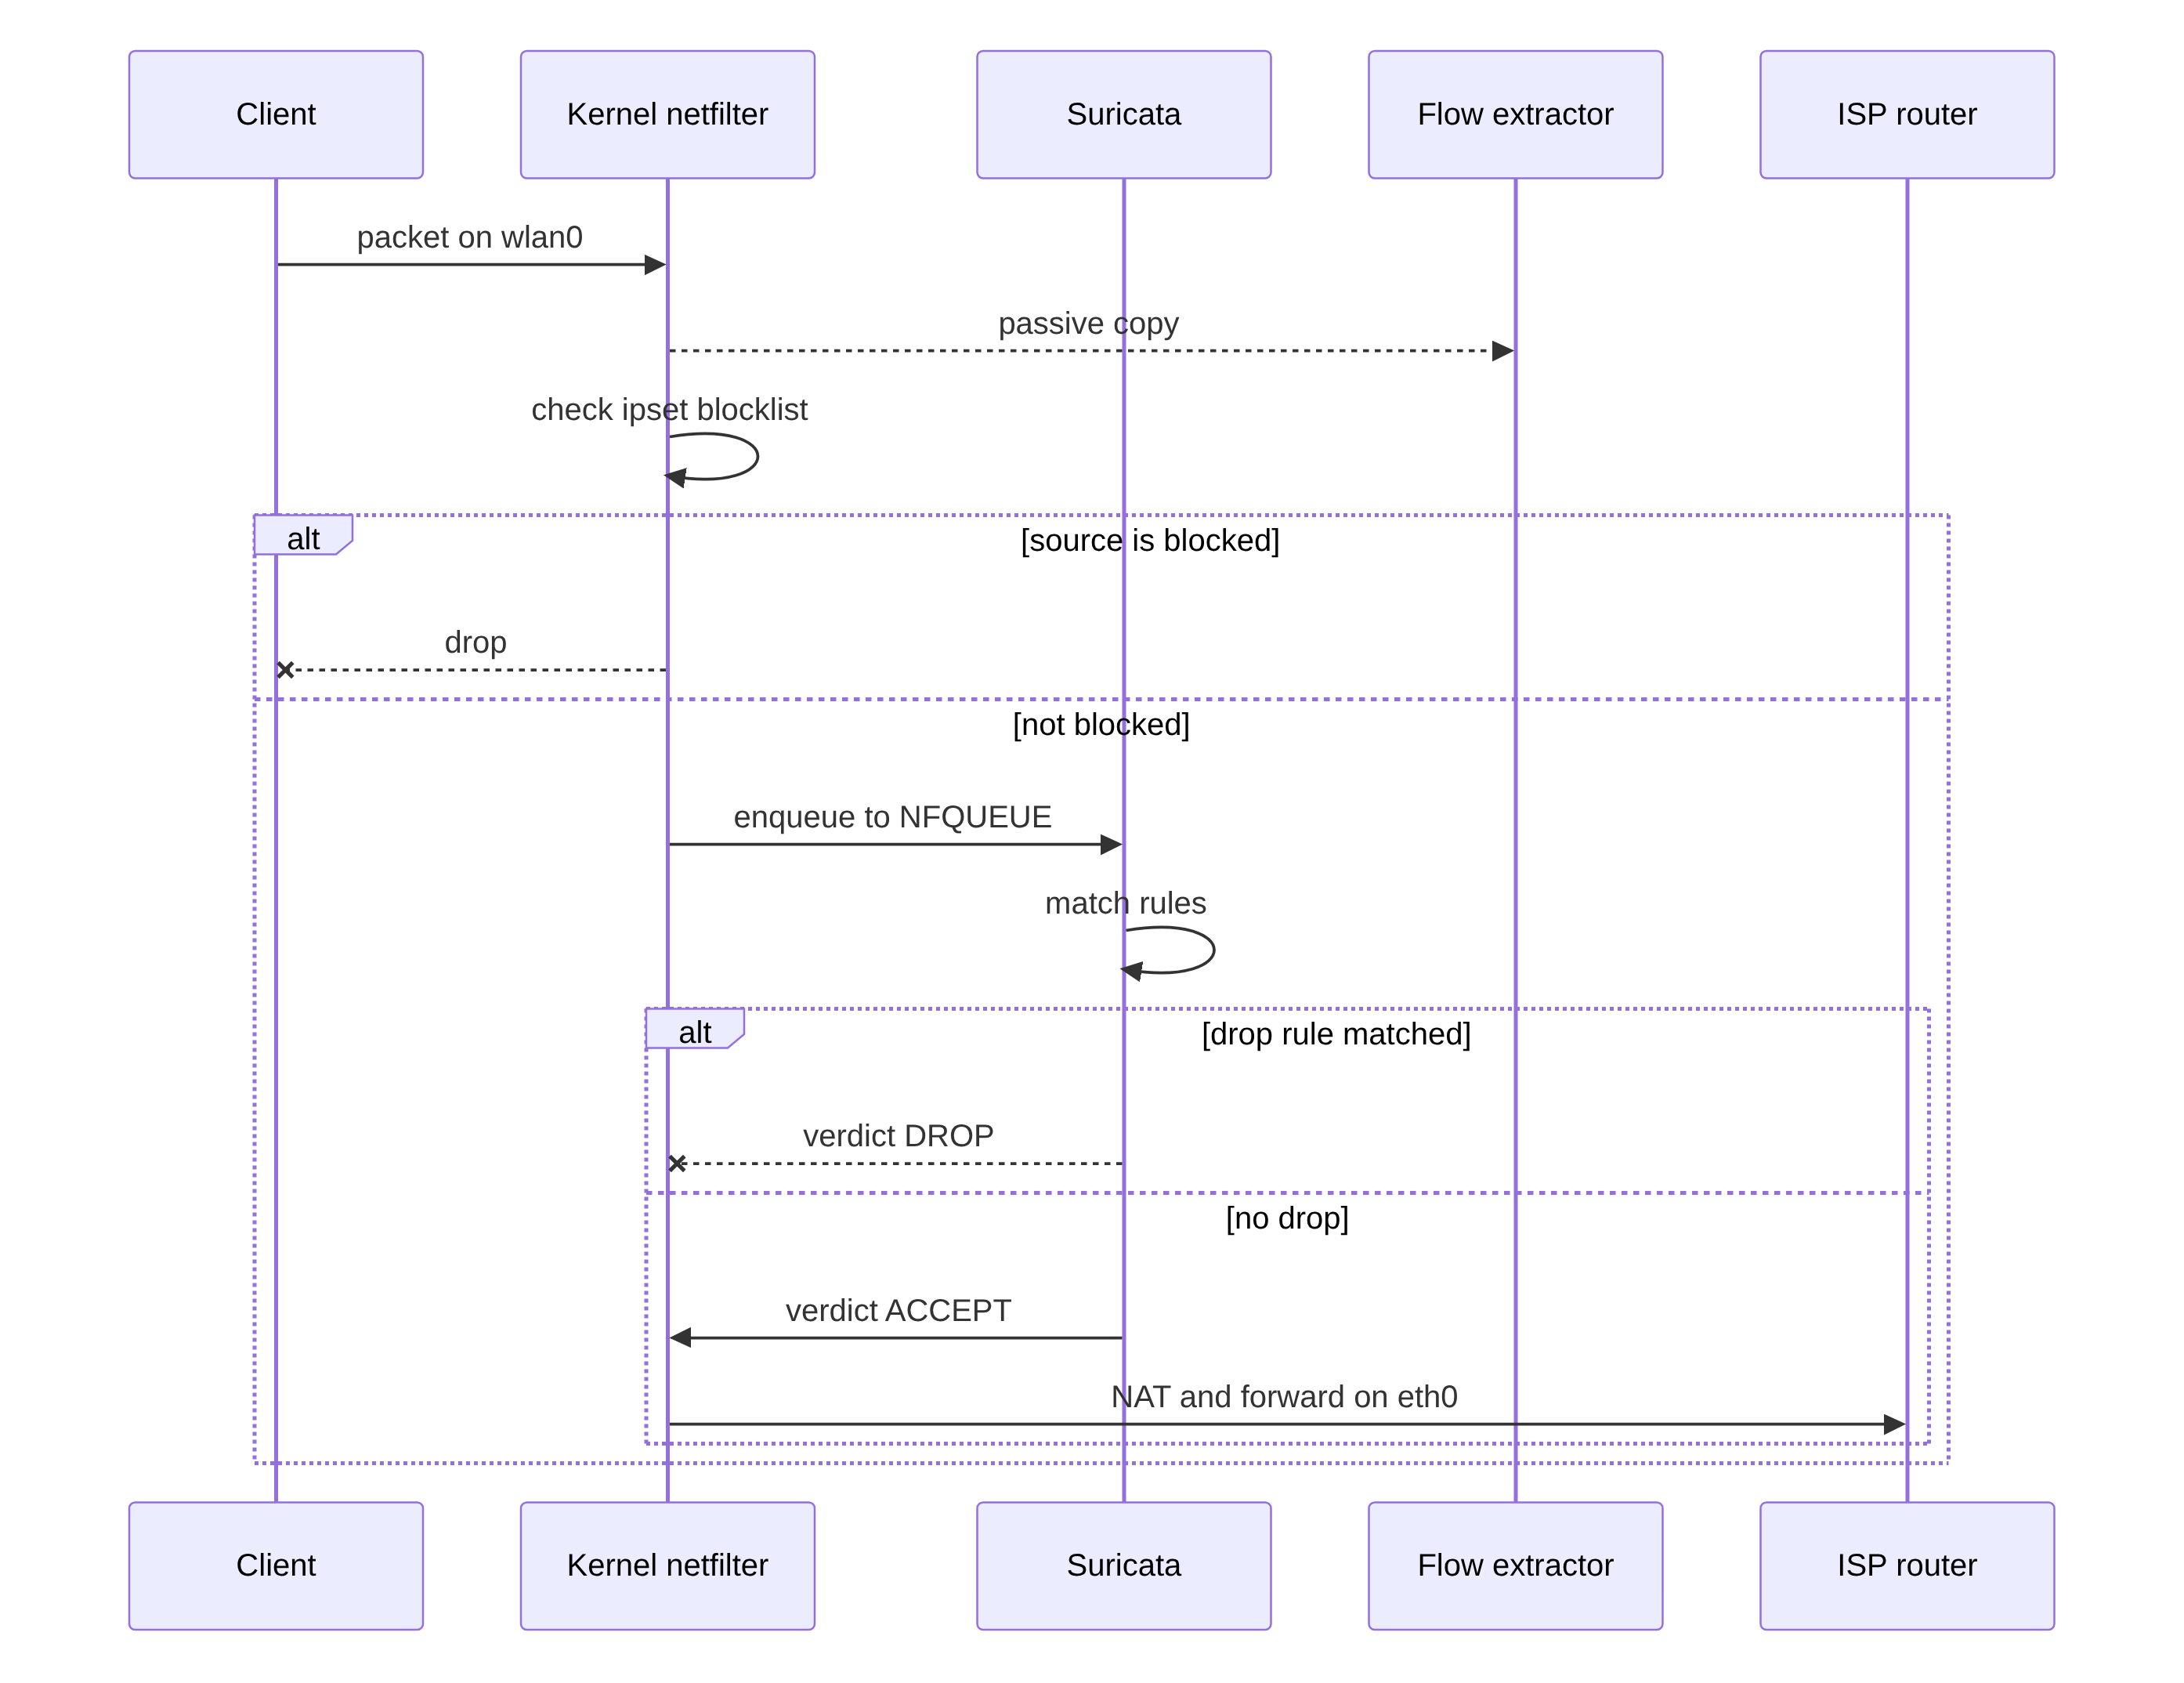
\includegraphics[width=0.85\textwidth]{Figures/nidps_fig6_2.png}
    \caption{Packet path through the data plane.}
    \label{fig:packetpath}
\end{figure}

\noindent The rule order matters: the ipset check comes before the queue, so packets from blocked hosts are discarded in the kernel and never cost Suricata any CPU. During a DDoS from a blocked source, this keeps the inspection engine free for other traffic.

\subsubsection{Detection Subsystem}\label{sec:6.3.1.2}
\noindent The detection subsystem has four producers. Suricata and the ARP monitor emit alerts directly. The flow extractor emits flow records, which the ML scorer enriches before publishing. Internally, the ML scorer is divided into three subcomponents:
\begin{itemize}
    \item \textbf{Feature validator:} checks each flow record against the model's feature schema and rejects mismatched or malformed records.
    \item \textbf{Flow models:} the Isolation Forest and the RF/XGBoost classifier, both loaded once at start-up and applied to every flow record.
    \item \textbf{Host behaviour tracker:} keeps per-host state (outbound byte baselines, per-key connection timestamps, local JA3 counts) and computes the exfiltration and beaconing scores of Sections~\ref{sec:exfil} and~\ref{sec:beacon}. Its state is bounded: entries for inactive hosts and keys expire.
\end{itemize}

\subsubsection{Decision and Response Subsystem}\label{sec:6.3.1.3}
\noindent The decision engine consumes all evidence from the bus, joins Suricata alerts with flow records by flow identifier and time, runs Algorithm~\ref{alg:verdict} and maintains the host scores of Section~\ref{sec:hostscore}. The enforcer receives BLOCK verdicts and runs Algorithm~\ref{alg:block}. The two are kept separate so that the component allowed to change firewall state is small, simple and easy to audit.

\subsubsection{Reliability Subsystem}\label{sec:6.3.1.4}
\noindent The watchdog receives heartbeats from every service and runs the state machine of Figure~\ref{fig:statemachine} for each. systemd provides process-level supervision (automatic restart, start order, resource limits), while the watchdog adds application-level health (queue depth, processing lag) and decides when to enter degraded mode. The kernel-level failure mode (queue bypass on or off) is set when the data plane starts, so it does not depend on the watchdog being alive.

\subsubsection{Management and Reporting Subsystem}\label{sec:6.3.1.5}
\noindent The dashboard API serves a web interface on the LAN side only. It provides live counters (flows per second, alerts and blocks per layer), an alert list with the evidence behind each verdict, the list of currently blocked hosts with a manual unblock action, host risk scores, component health, and configuration of thresholds, failure mode and allowlist. Configuration changes are validated, saved and published on the bus so running services pick them up without a restart.

\subsubsection{Offline Training Pipeline}\label{sec:6.3.1.6}
\noindent Figure~\ref{fig:training} shows the offline pipeline and the hand-over of models to the device.

\begin{figure}[!htbp]
    \centering
    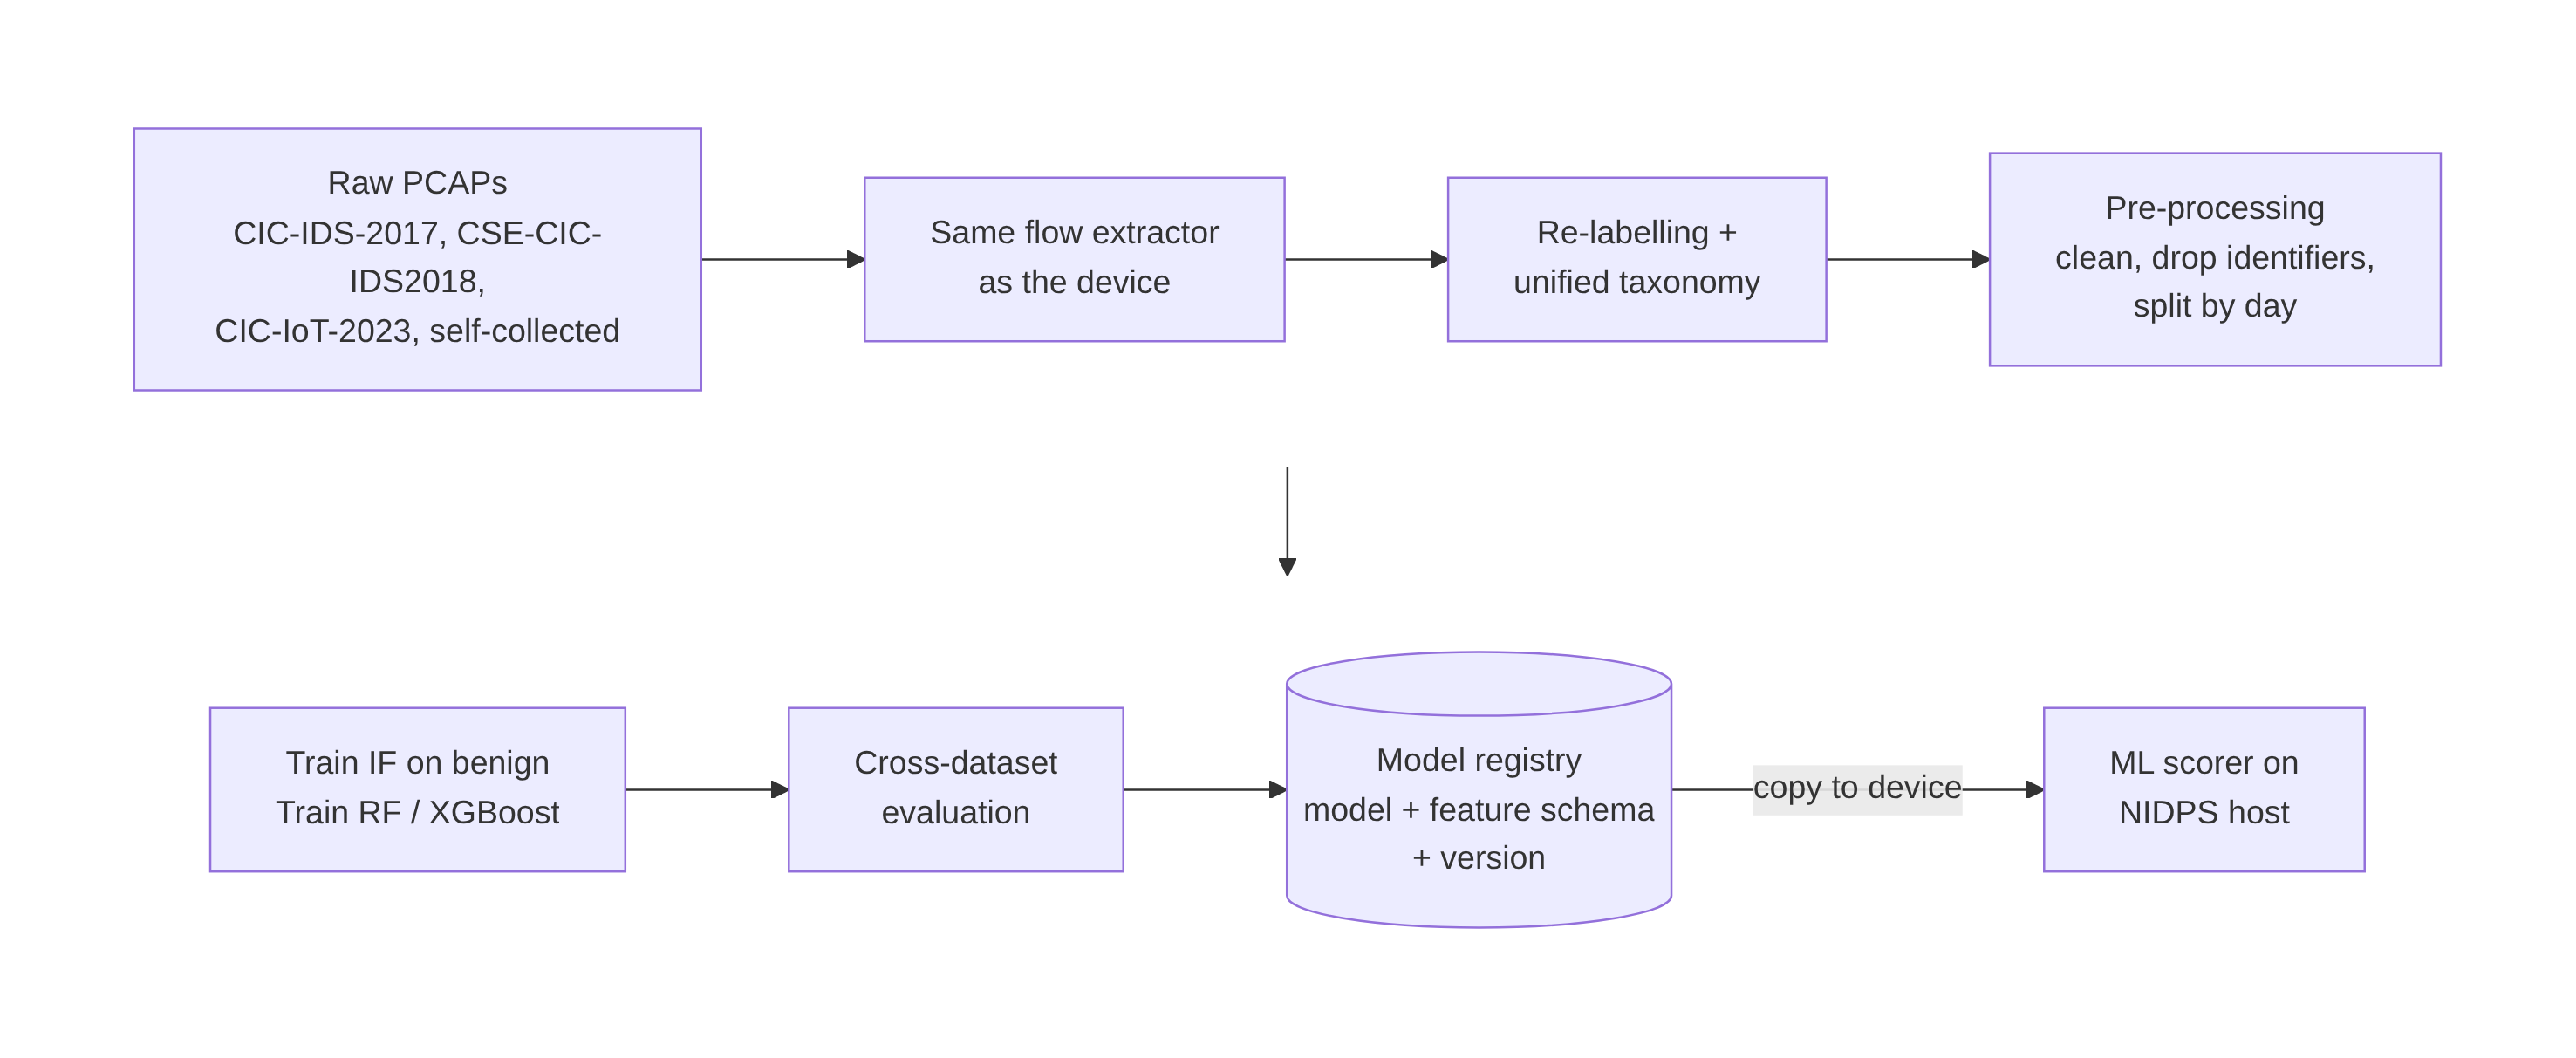
\includegraphics[width=0.9\textwidth]{Figures/nidps_fig6_3.png}
    \caption{Offline training pipeline and model hand-over to the device.}
    \label{fig:training}
\end{figure}

\noindent Training runs on a workstation, not on the NIDPS host, because it needs far more memory than inference. The only hand-over to the device is a model package containing the model file, its feature schema and a version manifest.

\section{Architectural Strategies}\label{sec:6.4}
\label{sec:archstrategies}
\noindent Each strategy below records the decision, the reasoning behind it and the alternatives that were rejected.

\subsection{Layered Defence with a Short Fast Path}\label{sec:6.4.1}
\noindent \textbf{Decision:} detection is split into a packet-level layer inside the forwarding path (Suricata) and flow-level layers outside it (ML), joined by a fusion step.

\noindent \textbf{Reasoning:} per-packet ML inference on every forwarded packet would exceed the CPU budget and add latency to every connection, violating the first goal of Section~\ref{sec:goals}. Flow-level ML outside the path costs nothing in forwarding latency, and Suricata covers the attacks that must be stopped at the first packet.

\noindent \textbf{Alternatives rejected:} ML-only inline detection (too slow, and no immediate protection against known attacks); Suricata-only detection (misses zero-day and behavioural attacks, the gap identified in Chapter~1).

\subsection{Metadata-Only Analysis of Encrypted Traffic}\label{sec:6.4.2}
\noindent \textbf{Decision:} encrypted traffic is analysed only through JA3/JA3S fingerprints and flow statistics.

\noindent \textbf{Reasoning:} TLS interception would require a trusted root certificate on every client, fails against certificate pinning, breaks some IoT devices outright and would multiply CPU load. It would also expose all household traffic in plain text on one device, which is a serious privacy risk.

\noindent \textbf{Alternatives rejected:} full TLS interception (above); ignoring encrypted traffic (most C2 now uses TLS). \textbf{Known limitation:} browsers now randomise TLS extension order, which makes JA3 less stable for browser traffic. Because fingerprinting is isolated in the flow extractor, it can be switched to JA4, which sorts extensions before hashing, without changing other components.

\subsection{Offline Training, Online Inference}\label{sec:6.4.3}
\noindent \textbf{Decision:} models are trained on a workstation and deployed as read-only, versioned packages. The device only performs inference and threshold calibration.

\noindent \textbf{Reasoning:} training on hundreds of millions of flows needs far more memory than the device has. Online retraining on the device would also let an attacker gradually teach the model that malicious traffic is normal (model poisoning). Recalibrating only the threshold (Section~\ref{sec:calibration}) adapts to the local network with bounded risk.

\noindent \textbf{Alternatives rejected:} continuous online learning (poisoning risk, hardware cost); a fixed global threshold (false positives on real home traffic).

\subsection{Local Services Connected by an Event Bus}\label{sec:6.4.4}
\noindent \textbf{Decision:} each component runs as its own systemd service, and components exchange messages through a local publish/subscribe bus. Redis Streams is the proposed implementation.

\noindent \textbf{Reasoning:} service isolation means a crash in one component does not take down the others, and systemd can restart each independently, which is a precondition for the failure modes. The bus decouples producers from consumers. Redis Streams is lightweight, keeps a bounded backlog that a restarted consumer can resume from, and supports consumer groups so the dashboard and the decision engine read the same events independently.

\noindent \textbf{Alternatives rejected:} direct function calls in one process (no fault isolation); Apache Kafka (far too heavy for the hardware); plain Unix sockets between each pair of components (simple, but every new consumer needs new wiring, and messages are lost while a consumer restarts). ZeroMQ was a close alternative and remains a fallback if Redis proves too heavy.

\subsection{Kernel-Enforced Blocking and Failure Semantics}\label{sec:6.4.5}
\noindent \textbf{Decision:} both blocking (ipset with timeouts) and the failure mode (NFQUEUE bypass or not) are enforced by the kernel, not by user-space software.

\noindent \textbf{Reasoning:} user-space components can crash; the kernel keeps running. Timed ipset entries expire even if the enforcer dies, so a crash never leaves hosts blocked forever, and the queue-bypass flag applies the chosen mode even if the watchdog is down.

\noindent \textbf{Alternatives rejected:} iptables rules added and deleted one per blocked host (slow with many entries and leaves stale rules after a crash); a user-space proxy that drops traffic (adds latency and is itself a crash risk).

\subsection{Choice of Languages and Products}\label{sec:6.4.6}
\noindent Table~\ref{tab:products} summarises the main product and language choices.

\begin{table}[H]
\centering
\caption{Product and language choices.}
\label{tab:products}
\begin{tabular}{|>{\raggedright\arraybackslash}p{0.13\linewidth}|>{\raggedright\arraybackslash}p{0.18\linewidth}|>{\raggedright\arraybackslash}p{0.3\linewidth}|>{\raggedright\arraybackslash}p{0.27\linewidth}|}
\hline
\textbf{Need} & \textbf{Choice} & \textbf{Main reason} & \textbf{Alternative considered} \\
\hline
Signature IPS & Suricata & Multi-threaded, native NFQUEUE IPS mode, EVE JSON output, TLS/JA3 support, maintained ET Open rules & Snort 3 (similar capability; Suricata chosen for its JSON output and threading) \\
\hline
Services and ML & Python 3 & scikit-learn and XGBoost available natively; fast development & C++ (faster, but much slower to develop; reconsidered only if profiling shows Python is the bottleneck) \\
\hline
Models & scikit-learn Isolation Forest and Random Forest, XGBoost & Small, fast tree models suited to tabular flow data & Deep autoencoders and LSTMs (higher compute cost, no clear gain on flow features) \\
\hline
Event store & SQLite & Zero administration, single file, enough for one device & PostgreSQL (needs a server process) \\
\hline
Dashboard & Python web API with WebSocket push and a lightweight web front end & Live updates with little code; reuses the Python stack & Grafana (heavy and less suited to showing verdict evidence and controls) \\
\hline
Firewall & iptables + ipset & Stated in the proposal; well documented; ipset handles large blocklists efficiently & nftables sets (modern equivalent; migration path kept open) \\
\hline
\end{tabular}
\end{table}

\subsection{Error Detection and Recovery}\label{sec:6.4.7}
\noindent Errors are handled at three levels.
\begin{enumerate}
    \item \textbf{Record level:} malformed flow records or alerts are rejected by the feature validator and counted, never passed to models.
    \item \textbf{Component level:} heartbeats and systemd supervision detect crashes and hangs and restart the component (Section~\ref{sec:failure}).
    \item \textbf{System level:} the kernel-enforced failure mode decides what happens to traffic while a component is down. All three levels log to the event store, so the dashboard can show when the system was not fully protected.
\end{enumerate}

\subsection{Data Storage, Persistence and Retention}\label{sec:6.4.8}
\label{sec:storage}
\noindent Only derived data is stored: alerts, verdicts, block records, host risk history, calibration state and configuration. Raw packets and payloads are never written to disk in normal operation. Flow records are kept for a short rolling window (for example, 7 days) for calibration and investigation, then deleted. This protects household privacy and keeps disk use bounded on a small device.

\subsection{Future Extension}\label{sec:6.4.9}
\noindent The architecture is designed so that the likely extensions require adding a component rather than changing existing ones: a new detector publishes to the bus; a new response (for example, notifying the owner's phone) subscribes to verdicts; a newer model or JA4 support is deployed as a new model package or extractor version.

\section{Domain Model/Class Diagram}\label{sec:6.5}
\label{sec:classdiagram}
\noindent Figure~\ref{fig:classdiagram} shows the main classes of the runtime system. The central entity is the Flow, which carries its features and optional TLS fingerprint through the pipeline. All detectors implement a common Detector interface and produce Evidence; the DecisionEngine turns Evidence into a Verdict, and the Enforcer turns BLOCK verdicts into BlockEntry records.

\begin{figure}[!htbp]
    \centering
    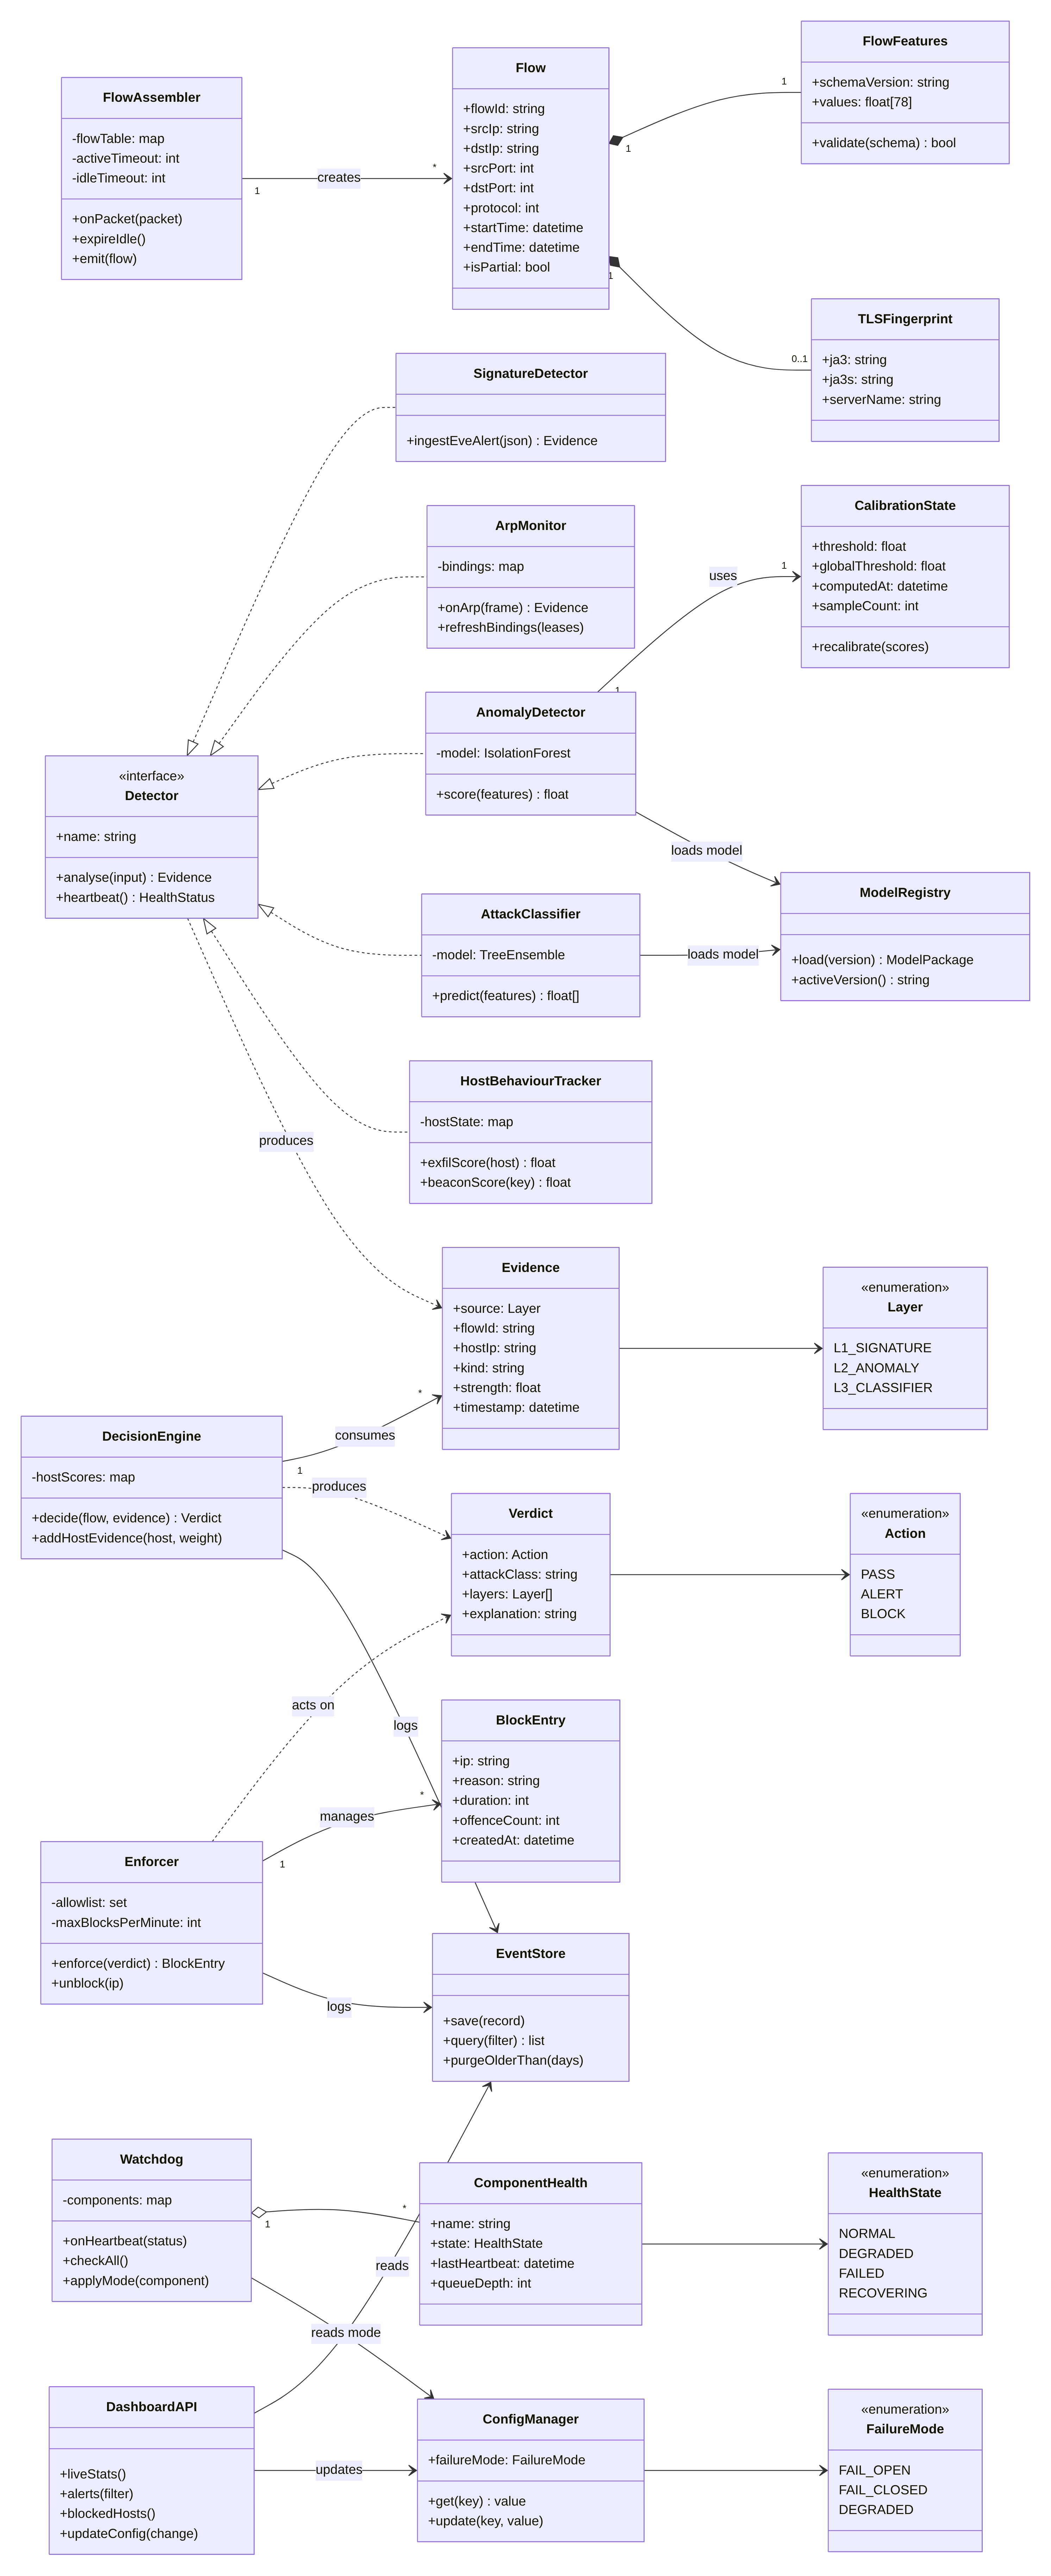
\includegraphics[height=0.85\textheight,keepaspectratio]{Figures/nidps_fig6_4.png}
    \caption{Class diagram of the NIDPS runtime.}
    \label{fig:classdiagram}
\end{figure}

\noindent The Detector interface is the main extension point: a new detection technique is added by implementing it and publishing its Evidence, without changes to the DecisionEngine. The Enforcer is the only class that changes firewall state, which keeps that responsibility in one small, auditable place.
\section{Policies and Tactics}\label{sec:6.6}
\label{sec:policies}
\noindent The following policies affect implementation details rather than the overall structure of the system.

\subsection{Rule and Threshold Management}\label{sec:6.6.1}
\noindent The ET Open ruleset is updated daily by a scheduled job, tested for syntax with Suricata's test mode, and loaded with a live rule reload so inspection never stops. If the test fails, the previous ruleset stays active. Custom rules live in a separate file under version control, so updates to ET rules never overwrite them. All numeric thresholds (rule thresholds, flow timeouts $T_a$ and $T_i$, $\tau$, $\theta$ values, $\Theta$, block durations) are read from one configuration file with documented defaults.

\subsection{Model Packaging and Versioning}\label{sec:6.6.2}
\label{sec:modelpackaging}
\noindent Each model package holds the model file, the ordered feature list with the extractor version, the class list and the training date and metrics. At load time the ML scorer refuses any package whose feature list does not match the running extractor. XGBoost models are stored in its native JSON format rather than as Python pickles, since loading a pickle can execute arbitrary code. scikit-learn models use joblib files, loaded only from the registry directory, which is writable only by the deployment user. The previous package is kept so a bad model can be rolled back with one command.

\subsection{Engineering Trade-offs}\label{sec:6.6.3}
\begin{itemize}
    \item \textbf{Detection speed vs.\ accuracy:} ML verdicts are per flow, not per packet (Section~\ref{sec:mltiming}), accepting a short delay for ML-detected attacks in exchange for zero added forwarding latency.
    \item \textbf{False positives vs.\ missed attacks:} the calibration percentile $p$ and the block thresholds are the explicit controls. Defaults lean towards fewer false positives, because wrong blocks on a home network cost the owner's trust quickly.
    \item \textbf{Availability vs.\ security:} chosen per deployment through the failure mode, with fail-open as the default for homes.
\end{itemize}

\subsection{Coding Guidelines and Conventions}\label{sec:6.6.4}
\noindent Python code follows PEP~8, uses type hints throughout and is checked with a linter and a type checker in continuous integration. Each service is a separate package with a single entry point. Messages on the event bus use a versioned JSON schema, so producers and consumers can be upgraded independently. Logs are structured JSON with a timestamp, component name and flow or host identifier, so events can be traced across services.

\subsection{Requirements Traceability}\label{sec:6.6.5}
\noindent Every goal from Chapter~\ref{chap:2} is mapped to the components that implement it and the tests that verify it, in a traceability matrix kept in the repository and updated at every sprint review (Table~\ref{tab:traceability}).

\begin{table}[H]
\centering
\caption{Requirements traceability matrix.}
\label{tab:traceability}
{\small
\begin{tabular}{|>{\raggedright\arraybackslash}p{0.3\linewidth}|>{\raggedright\arraybackslash}p{0.3\linewidth}|>{\raggedright\arraybackslash}p{0.3\linewidth}|}
\hline
\textbf{Proposal objective} & \textbf{Implemented by} & \textbf{Verified by} \\
\hline
Transparent inline NIDPS between clients and ISP gateway & Data plane (Section~\ref{sec:subsysarch}) & Connectivity and latency tests (Table~\ref{tab:sysperf}) \\
\hline
Suricata with ET ruleset for known attacks & SignatureDetector, custom rules (Section~\ref{sec:layer1}) & Live attack replay: SSH brute force, port scan, DNS spoofing \\
\hline
ML pipeline for anomaly detection and classification & AnomalyDetector, AttackClassifier, HostBehaviourTracker (Sections~\ref{sec:layer2}--\ref{sec:layer3}) & Detection metrics and live replay: C2 beaconing, exfiltration, DDoS, lateral movement \\
\hline
Cross-evaluation on three public datasets & Offline training pipeline (Figure~\ref{fig:training}) & Cross-dataset matrix (Table~\ref{tab:crossmatrix}) \\
\hline
Automatic blocking via iptables & Enforcer (Section~\ref{sec:prevention}) & Time-to-block measurement; allowlist and rate-limit tests \\
\hline
Watchdog and configurable failure handling & Watchdog, systemd units (Section~\ref{sec:failure}) & Fault-injection tests in each failure mode \\
\hline
Web dashboard & DashboardAPI (Section~\ref{sec:subsysarch}) & Functional UI tests; usability check with non-expert users \\
\hline
\end{tabular}
}
\end{table}

\subsection{Testing Plan}\label{sec:6.6.6}
\begin{enumerate}
    \item \textbf{Unit tests} for each algorithm: flow assembly on crafted PCAPs, JA3 computation against published reference hashes, threshold calibration, fusion rules and the enforcer's allowlist, rate limit and back-off.
    \item \textbf{Integration tests} that replay labelled PCAPs through the full pipeline on a test host and compare verdicts with labels.
    \item \textbf{Live attack tests} on the isolated lab network, executing each in-scope attack from the attacker machine against our own test devices.
    \item \textbf{Performance tests} for latency, throughput and resource use (Table~\ref{tab:sysperf}).
    \item \textbf{Fault-injection tests:} each service is killed or frozen under load in each failure mode, and recovery time and traffic impact are recorded.
    \item \textbf{Soak test:} the system runs for at least one week on a real home network in alert-only mode to measure false positives before blocking is enabled.
\end{enumerate}

\subsection{Hierarchical Organisation of the Source Code}\label{sec:6.6.7}
\noindent The source code is organised as follows:
{\footnotesize
\begin{verbatim}
nidps/
  dataplane/      hostapd, dnsmasq and netfilter configuration + setup scripts
  suricata/       suricata.yaml, custom.rules, rule-update job
  services/
    arpmon/       ARP consistency monitor
    flowextract/  flow assembler, feature computation, JA3/JA3S
    mlscorer/     feature validator, models, host behaviour tracker, calibration
    decision/     decision engine and host scores
    enforcer/     ipset management, allowlist, back-off
    watchdog/     heartbeat monitoring, state machine, failure modes
    dashboard/    web API and front end
  common/         bus client, message schemas, config loader, logging
  training/       dataset builder, labelling, training and evaluation scripts
  models/         model registry (versioned packages)
  deploy/         systemd unit files, install and upgrade scripts
  tests/          unit, integration, fault-injection tests and test PCAPs
  docs/           traceability matrix, design notes
\end{verbatim}
}

\subsection{Build and Deployment}\label{sec:6.6.8}
\noindent The system is installed on a fresh Debian-based image by one installation script that installs system packages (Suricata, hostapd, dnsmasq, ipset, Redis), creates a Python virtual environment with pinned dependency versions, copies the configuration and the active model package, and enables the systemd units in dependency order: data plane first, then Suricata, then the remaining services. Upgrades replace one service at a time and restart only that service. Because every service is supervised and the failure mode is kernel-enforced, an upgrade never leaves the network without a defined behaviour.

\subsection{Maintenance}\label{sec:6.6.9}
\noindent Routine maintenance is automated: daily rule updates, weekly threshold recalibration (Algorithm~\ref{alg:calibration}), and log and flow-record purging beyond the retention window. Models are retrained offline when new datasets or significant new attack classes become available, or when the dashboard shows a rising alert rate that calibration does not explain. Component health history on the dashboard tells the owner when the system has been running in a degraded or failed state.

\section{Conclusion}\label{sec:6.7}
\label{sec:ch6conclusion}
\noindent This chapter translated the methodology of Chapter~\ref{chap:approach} into a concrete design. The NIDPS is a single Linux host organised as five runtime subsystems (data plane, detection, decision and response, management and reporting, and reliability) plus an offline training pipeline. The main architectural decisions keep the forwarding path short, analyse encrypted traffic only through metadata, train offline while calibrating thresholds online, isolate components as supervised services connected by an event bus, and let the kernel enforce both blocking and failure behaviour. The class diagram defines a common Detector interface that makes new detectors easy to add, while confining firewall changes to a single Enforcer. The policies on rule and model management, testing, traceability and deployment complete the design and connect each proposal objective to the component that delivers it and the test that verifies it.
